%%%%%%%%%%%%%%%%% TASK 1 %%%
\section{Image Processing for Earth Observation}

\subsection{Space Imagery}

\subsection{Computer Vision}

\subsection{Filtering}

\subsection{Image Processing \& Analysis}

\subsection{Pattern Recognition}

\subsection{Geometry}


%%%%%%%%%%%%%%%%% TASK 3 %%%
\section{Computer Vision \& Morphology}

\subsection{Erosion \& Dilatation}

\subsection{Morphological Filtering}

\subsection{Morphological Skeletonization \& Segmentation}


%%%%%%%%%%%%%%%%% TASK 3 %%%
\section{Data Analysis \& Processing}
After having extensively discussed Image Processing and Image Analysis in the previous chapters we will now move on to Data Analysis. \\In general, Data Analysis is an extension or generalisation of Image Analysis - in particular, an image can also be seen as a set of data with a specific topology. However, data analysis is not limited to images but can be used for a vast amount of applications, be it business, science or others, where a set of data is given and information has to be extracted. Ultimately, this is the goal of data analysis: shaping, modelling and analysing the data to gain information or conclusions from given data.
Since this course puts an emphasis on analysing and processing images, all the following examples will be performed on and explained by using images as a data set.

The term \textit{data} itself can be interpreted and defined in multiple ways, which raises the need for a definition in our context of data analysis of images.
In general data can be considered as an element taken from a set of data-elements. Each data-element can then be seen as a set of different components, attributes, parameters etc. - defining what the data-element is composed of - and are often called \textit{descriptors}. Mathematically speaking, this means that our data $\boldsymbol{x}$ is associated to a vector in $\boldsymbol{\mathbb{R}^n}$ containing the descriptors,
\begin{equation*}
	x = (c_1 ... c_n)^T
\end{equation*}
which is also called the \textit{state space E} of our data.
These descriptors are the crucial part when analysing data, since they are defining a set of rules according to which we analyse the raw data.

If this terminology is applied to images, the pixels or a range of pixels in each image can be seen as such an descriptor, thus the image itself as our data-element.

\subsection{Classification}
\begin{figure}[h!]
	\centering
	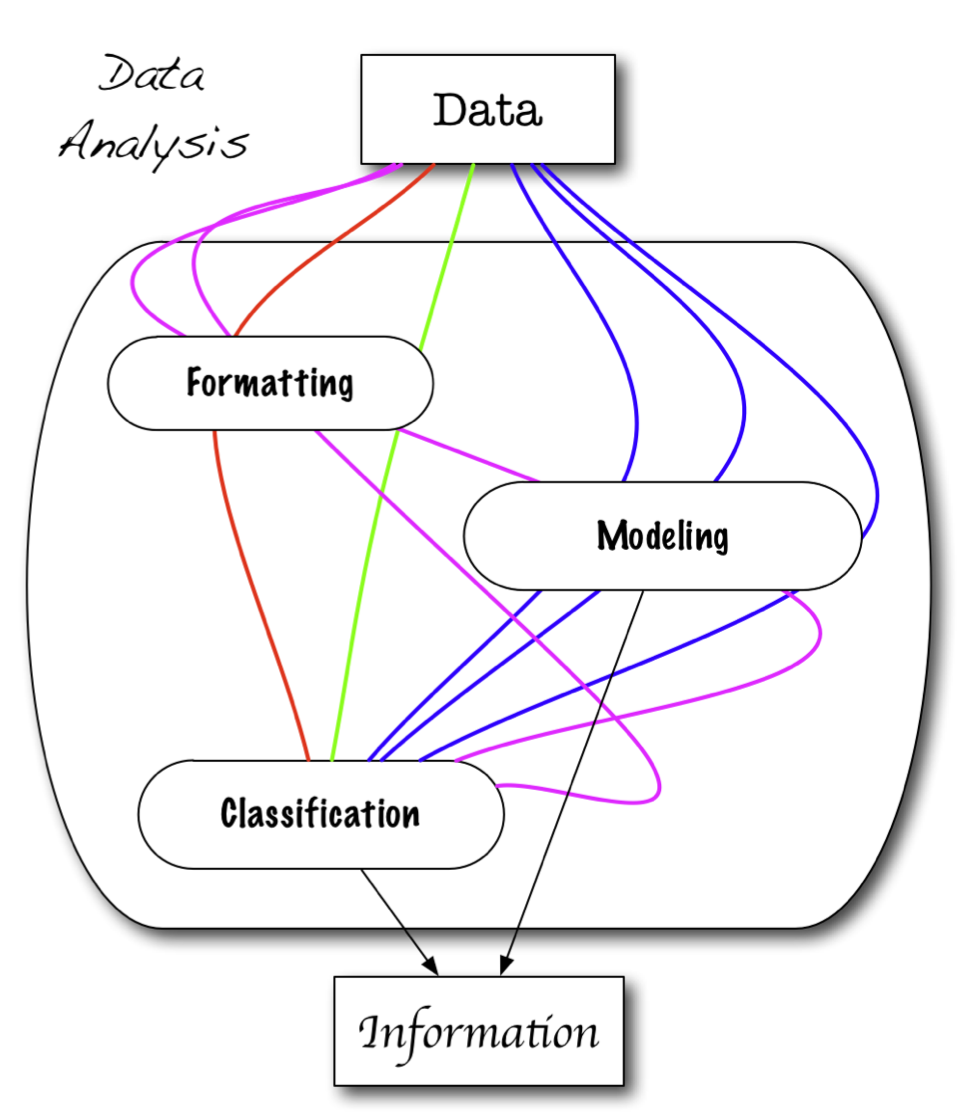
\includegraphics[width=\textwidth/2-5em]{images/data_analysis.png}
	\caption{Steps for classification \protect\footnotemark}
	\label{fig:data_anal}
\end{figure}
\footnotetext{source: lecture notes by Emmanuel Zenou}
Having a data set that consists of descriptors essentially allows us to \textit{label} this particular data set. This labelling of data is usually also described as \textit{Classification}, meaning that each data-element or sub-data-element is assigned a particular \textit{class}. In image analysis for space applications typically the pixels in an image have to be classified.

In general, classification of data consists of three steps,
\begin{enumerate}
	\item Formatting
	\item Modelling
	\item Classification
\end{enumerate}
whereas these steps are not compulsory. The formatting step usually consists of finding good descriptors, changing the state space (e.g. by re-shaping), pre-processing data (e.g. filtering) and so on.\\
The modelling step requires to find a model and its optimal parameters to fit the data, but also to fit the model output to the data and to validate the model.
In the final Classification part, the task is to find classes and a classification rule according to which distinct data will be labeled.

There are two main forms of classification, \textit{Supervised} and \textit{Unsupervised}, of which both are described and explained in detail in the following chapters.


\subsection{Supervised Classification}
Supervised Classification describes a technique, where the classes a data-set contains is known before starting the classification process. This, however, requires a human or another classification algorithm to properly detect and label desired features in either the same or similar images, which implies high effort on pre-processing and preparing the data sets.\\
For this particular technique there is a great amount of algorithms available, be it kNN, Maximum Likelihood, Bayesian or Linear Classification, Support Vector Machines or Neural Networks. During the laboratory we focused on the kNN algorithm and neural networks in particular, which is why the following sections will provide examples using these techniques.

\subsubsection{k - Nearest Neighbour}

The \textit{k - Nearest Neighbour} algorithm is the most simple classification algorithm in the supervised classification domain. 

\begin{figure}[h!]
	\centering
	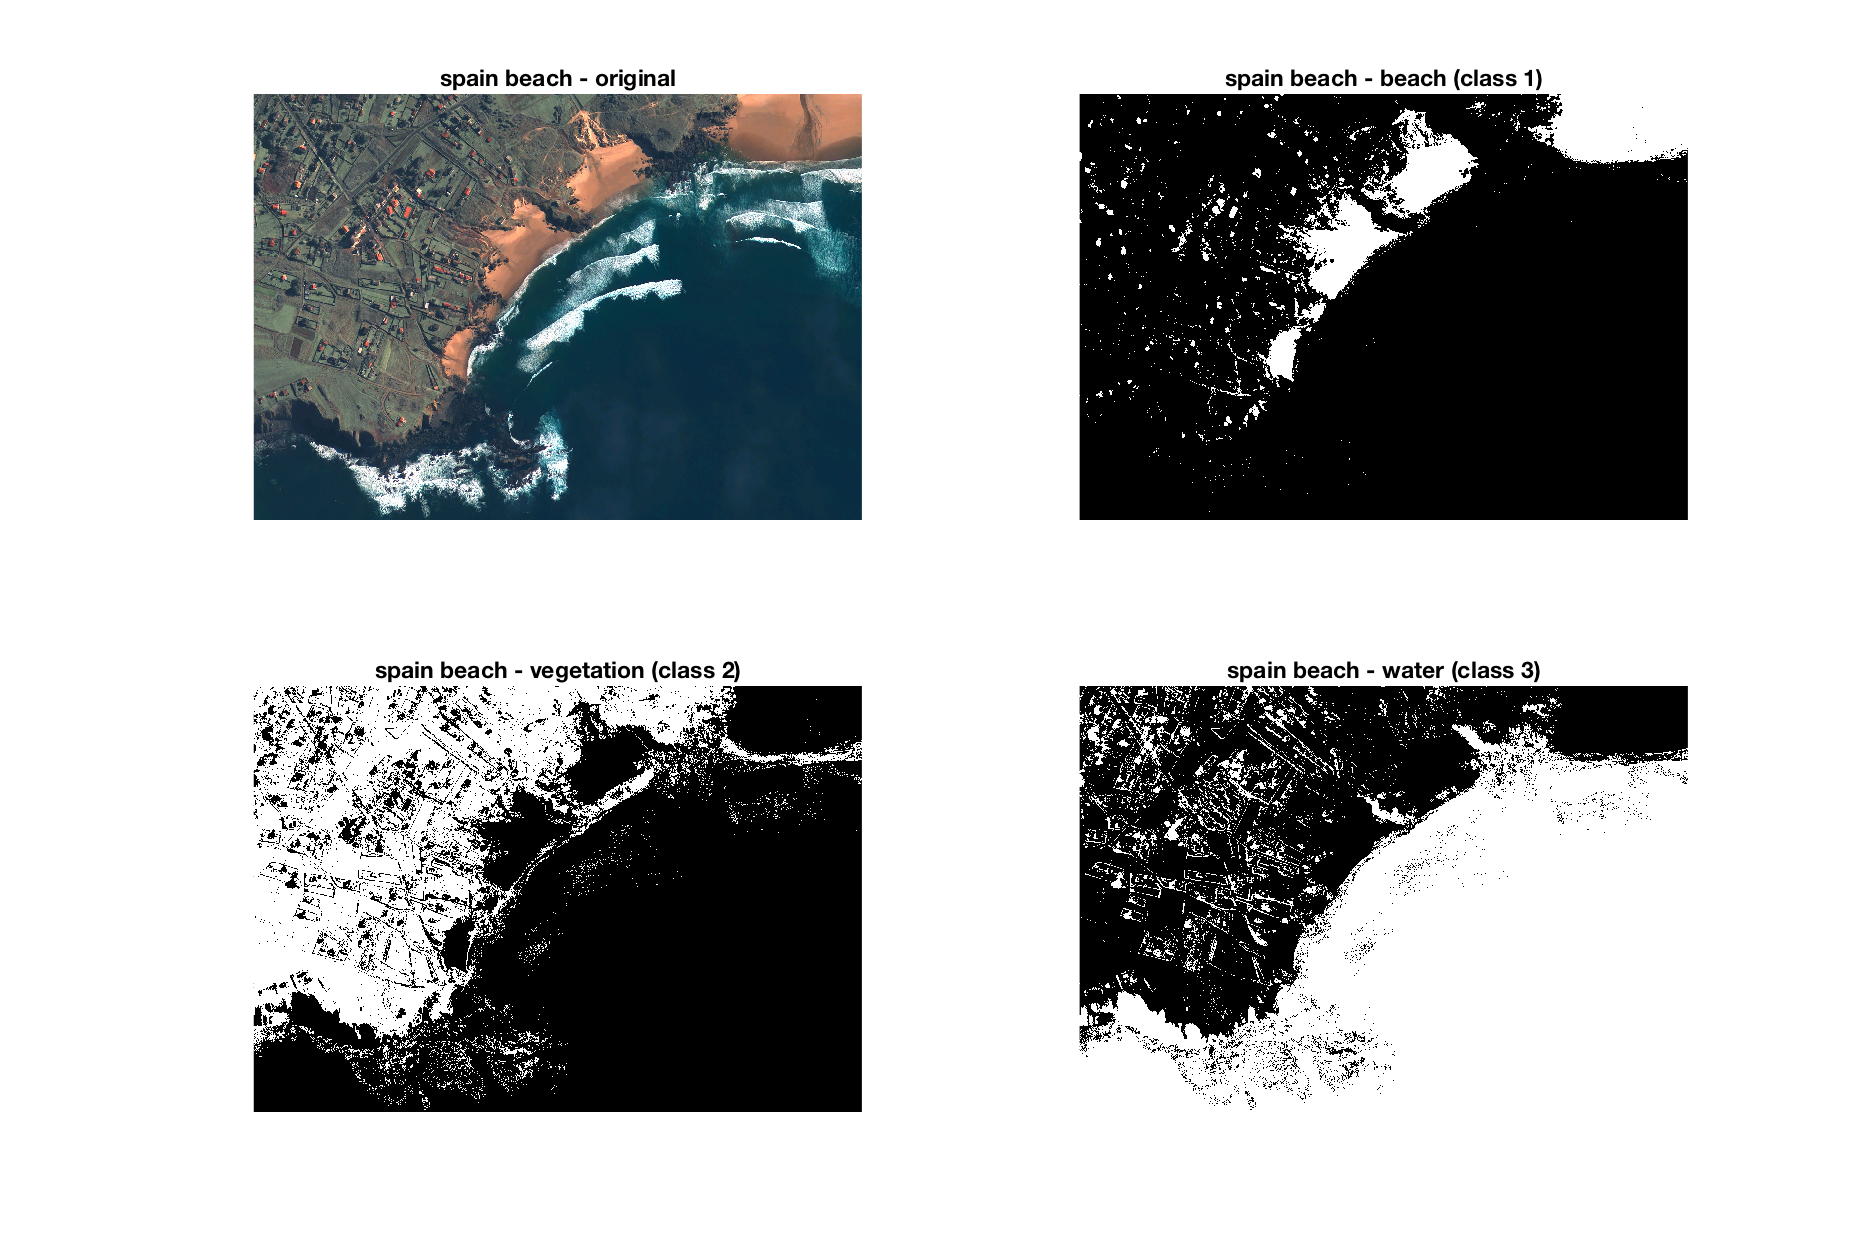
\includegraphics[width=\textwidth]{images/kNN.png}
	\caption{kNN algorithm applied on three classes}
	\label{fig:kNN}
\end{figure}

The underlying principle is to find the \textit{k} nearest neighbours to given data, to determine the class of it - which basically results in a calculation of distance. One way to apply this technique to images is to get the desired RGB values of pixels (e.g. by selecting pixels by hand at the desired image feature) and let the algorithm compare the pixels in an image to this particular RGB value.\\
This can be done of course for a range of RGB values, as is demonstrated in \cref{fig:kNN}, where an image was analysed with respect to three different classes: beach, vegetation and water. For each of these classes RGB values were taken and then used to compare the rest of the image to them. The appropriate MATLAB Code can be found in \cref{apdx:kNN}. Still, it is easy to see that this approach is not perfect. First, it requires to preprocess the image by choosing RGB values. Second, the output images are not perfect in terms of recognising the actual image features we wanted, e.g. when "detecting" water, there are a lot of points recognised on the land-part of the image, since the color is similar.


\subsubsection{Neural Networks}
A different approach of classifying data is using neural networks.

\subsection{Unsupervised Classification}
